%%%%%%%%%%%%%%%%%%%%%%%%%%%%%%%%%%%%%%%%%%%%%%%%%%%%%%%%%%%%%%%%%%%%
%% I, the copyright holder of this work, release this work into the
%% public domain. This applies worldwide. In some countries this may
%% not be legally possible; if so: I grant anyone the right to use
%% this work for any purpose, without any conditions, unless such
%% conditions are required by law.
%%%%%%%%%%%%%%%%%%%%%%%%%%%%%%%%%%%%%%%%%%%%%%%%%%%%%%%%%%%%%%%%%%%%
\documentclass{beamer}

\usepackage[english]{babel}
\usepackage[utf8]{inputenc}
\usepackage[T1]{fontenc}
\usepackage{booktabs}
\usetheme[workplace=ics]{MU}



% %% These macros specify information about the presentation
% \title{Walsh functions for high-resolution shock capturing and their applications to expansion tube simulations} %% that will be typeset on the
% \subtitle{Confirmation Seminar} %% title page.
% \author{Jamie Border}


% %% These additional packages are used within the document:
% \usepackage{ragged2e}  % `\justifying` text
% \usepackage{booktabs}  % Tables
% \usepackage{tabularx}
% \usepackage{tikz}      % Diagrams
% \usetikzlibrary{calc, shapes, backgrounds}
% \usepackage{amsmath, amssymb}
% \usepackage{url}       % `\url`s
% \usepackage{listings}  % Code listings
% \frenchspacing

% added by Jamie
\usepackage{bbding}
% \setbeamertemplate{itemize items}[square]
\newcommand\Wider[2][3em]{%
\makebox[\linewidth][c]{%
  \begin{minipage}{\dimexpr\textwidth+#1\relax}
  \raggedright#2
  \end{minipage}%
  }%
}
\usepackage{multimedia}
% \usefonttheme[onlymath]{serif}
% \usefonttheme{professionalfonts}
\usepackage{framed}
\newcommand{\mybox}[3]{{\color{#1}\framebox{\color{#2}#3}}}
\usepackage[skins,listings,breakable,many]{tcolorbox}
% \lstset{basicstyle=\footnotesize, columns=fullflexible}
% \lstset{basicstyle=\footnotesize, backgroundcolor=\color{lightgray}}
% \lstset{basicstyle=\footnotesize, showstringspaces=false}
\lstset{basicstyle=\scriptsize, showstringspaces=false}
\usepackage{ulem}

\newcommand\blfootnote[1]{%
  \begingroup
  \renewcommand\thefootnote{}\footnote{#1}%
  \addtocounter{footnote}{-1}%
  \endgroup
}

\begin{document}

\title[]{\sout{NCI Australia's} Jamie's GPU Hackathon} %% that will be typeset on the
\subtitle[]{A lightning talk} %% title page.
\author[]{Jamie Border}
% \title[Short Presentation Title]{Full Presentation Title}
% \subtitle[Short Presentation Subtitle]{Full Presentation Subtitle}
% \author[J.\,Doe]{Jane Doe \\ personal-id@mail.muni.cz}
\institute{School of Mechanical and Mining Engineering, The University of Queensland}
\date{August 26th, 2020}
% \date{\today}
% \subject{Presentation Subject}
% \keywords{the, presentation, keywords}

% \begin{frame}[plain]
% \maketitle
% \end{frame}
  \frame{\maketitle}
  % \maketitle


  % \begin{darkframes}

    % Stability Analysis
    %%%%%%%%%%%%%%%%%%%%%%%%%%%%%%%%%%%%%%%%%%%%%%%%%%%%%%%%%%%%%%%%%%%%%
    % \begin{frame}{\mybox{mubeamer@base}{blue}{Title}}
    % \begin{frame}{\mybox{mubeamer@gray5}{blue}{Title}}
    % \begin{frame}{\mybox{mubeamer@orange1}{blue}{Title}}
    % \begin{frame}{\mybox{mubeamer@ped}{blue}{Title}}
    % \begin{frame}{\mybox{mubeamer@sci}{blue}{Title}}
    % \begin{frame}{\mybox{mubeamer@fsps}{blue}{Title}}
    % \begin{frame}{\mybox{red}{blue}{Title}}
    % \framesubtitle{}
        % some text here
    % \end{frame}
    %%%%%%%%%%%%%%%%%%%%%%%%%%%%%%%%%%%%%%%%%%%%%%%%%%%%%%%%%%%%%%%%%%%%%

    % Workflow Analysis
    %%%%%%%%%%%%%%%%%%%%%%%%%%%%%%%%%%%%%%%%%%%%%%%%%%%%%%%%%%%%%%%%%%%%%
      % Reproducibility crisis in scientific community 
      % - not as much of an issue for engineering, but still good to be able to easily replicate your own work)
      % WET vs DRY programing principles
      % Intro to makefiles 
      % Intro to bash scripts
      % Intro to python with os module
      % Intro to gnuplot
      % putting it all together, demonstration
      
    \begin{frame}{\mybox{red}{blue}{Why so slow?}}
    \framesubtitle{}
        % \begin{itemize}
            % \item My experience is with CUDA Fortran
            % \item Very little C++ experience, no CUDA C experience
            % \item No experience linking D with C/C++
        % \end{itemize}
        \begin{figure}
            \colorbox{white}{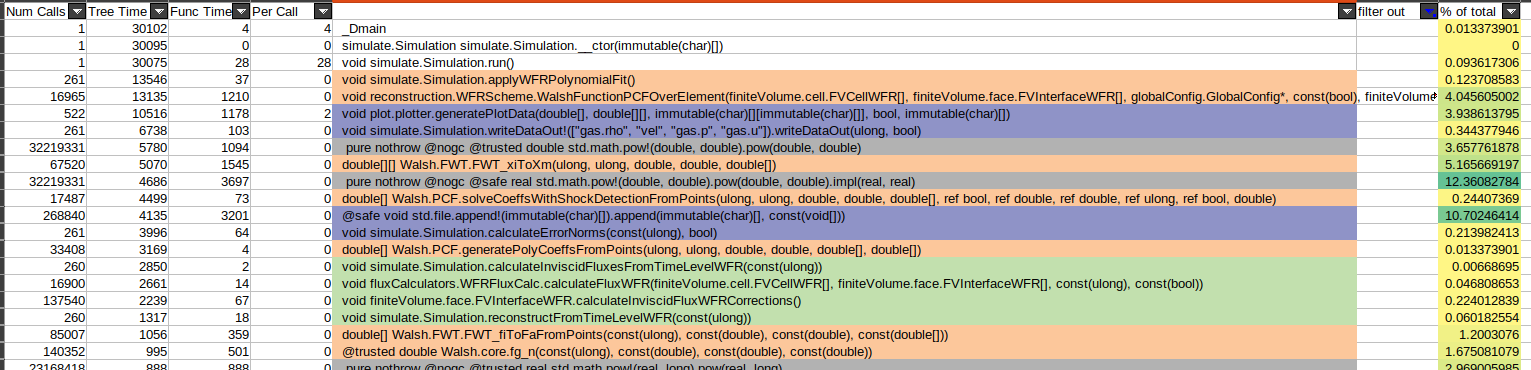
\includegraphics[width=0.9\textwidth,trim=0 0 0 0,clip]{profile.png}}
            % \caption{}
        \end{figure}
        \vspace{-1.0cm}
        % \hspace{-4.0cm}
        \begin{columns}[t]
            \begin{column}{0.2\textwidth}
        \begin{figure}
            \colorbox{white}{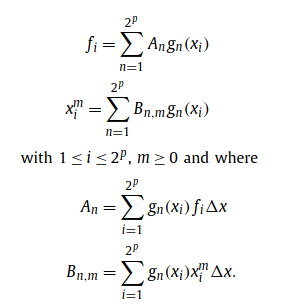
\includegraphics[width=1.2\textwidth,trim=0 0 0 0,clip]{eqs.png}}
            % \caption{}
        \end{figure}
            \end{column}
            \vspace{-1.0cm}
            % \hspace{-2.0cm}
            \begin{column}{0.3\textwidth}
        \begin{figure}
            \colorbox{white}{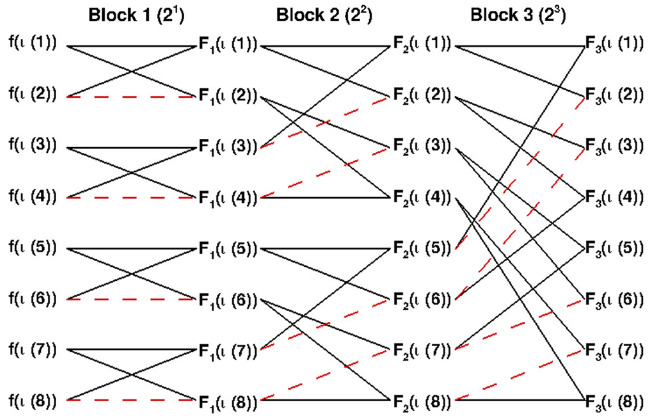
\includegraphics[width=1.2\textwidth,trim=0 0 0 0,clip]{seq_ordered_FWT.png}}
            % \caption{}
        \end{figure}
            \end{column}
            % \hspace{1.0cm}
            \begin{column}{0.4\textwidth}
                \vspace{0.5cm}
        \begin{figure}
            \colorbox{white}{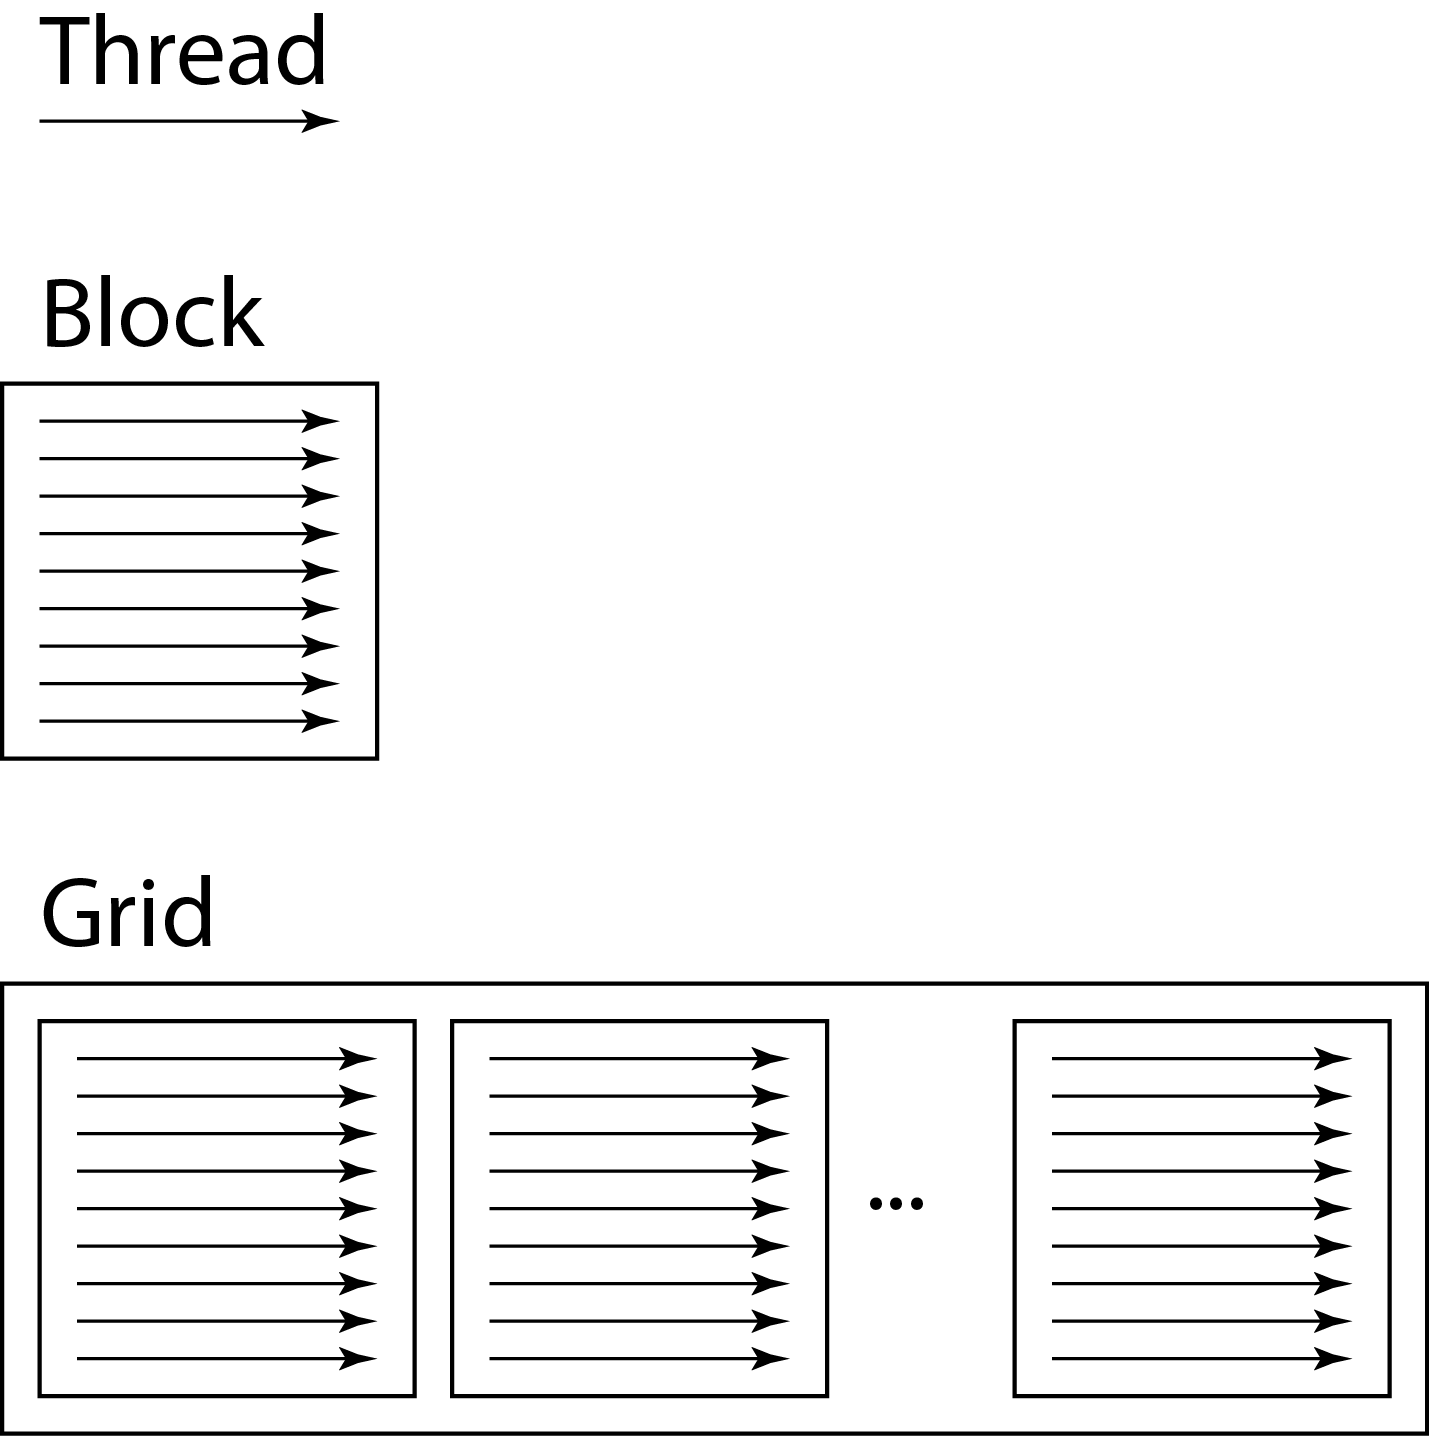
\includegraphics[width=0.6\textwidth,trim=0 0 0 0,clip]{cudastructure.png}}
            % \caption{}
        \end{figure}
            \end{column}
        \end{columns}
    \end{frame}

    \begin{frame}[fragile]{\mybox{red}{blue}{CUDA C Kernel}}
    \framesubtitle{}
        \vspace{-1.2cm}
        \begin{columns}[t]
            \begin{column}{0.3\textwidth}
        \begin{figure}
            \colorbox{white}{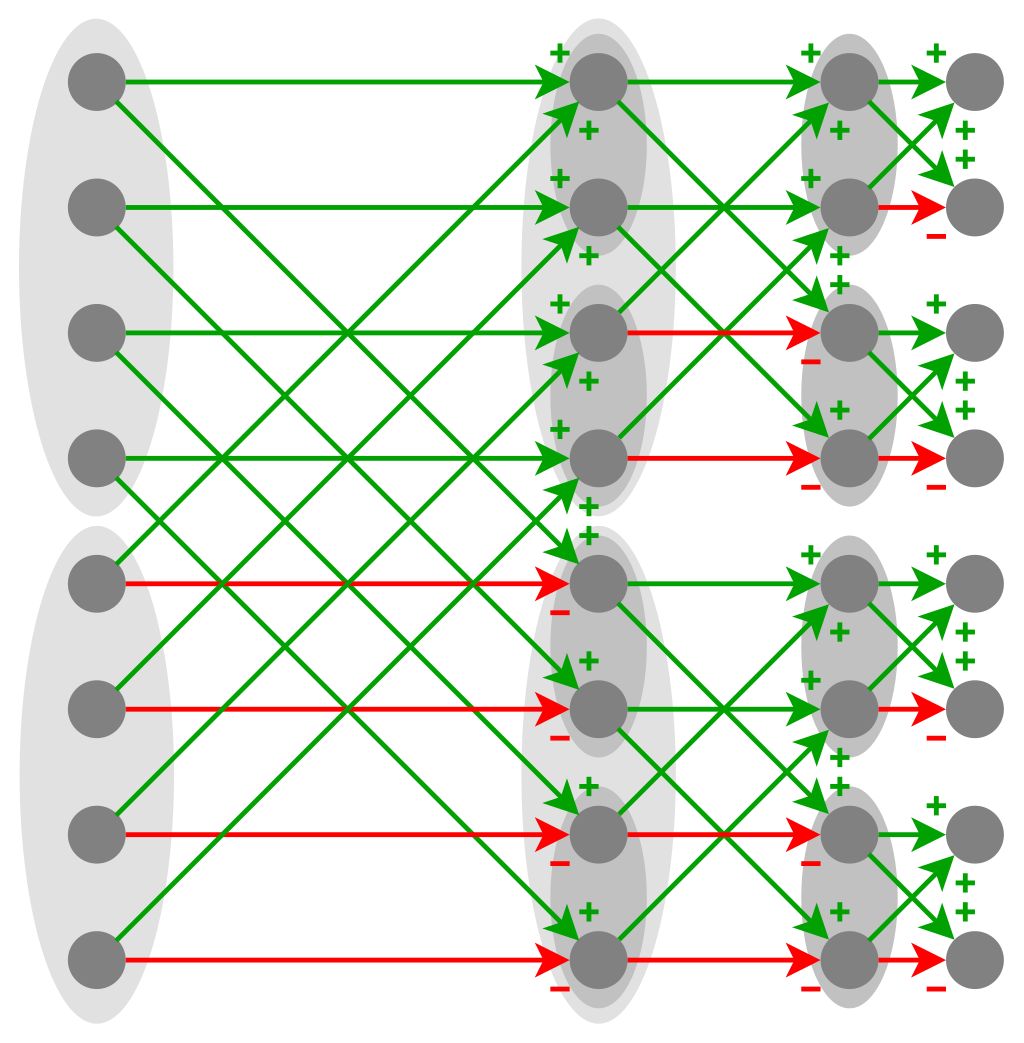
\includegraphics[width=1.0\textwidth,trim=0 0 0 0,clip]{wht.png}}
            % \caption{}
        \end{figure}
        \vspace{-0.2cm}
        \begin{figure}
            % \colorbox{white}{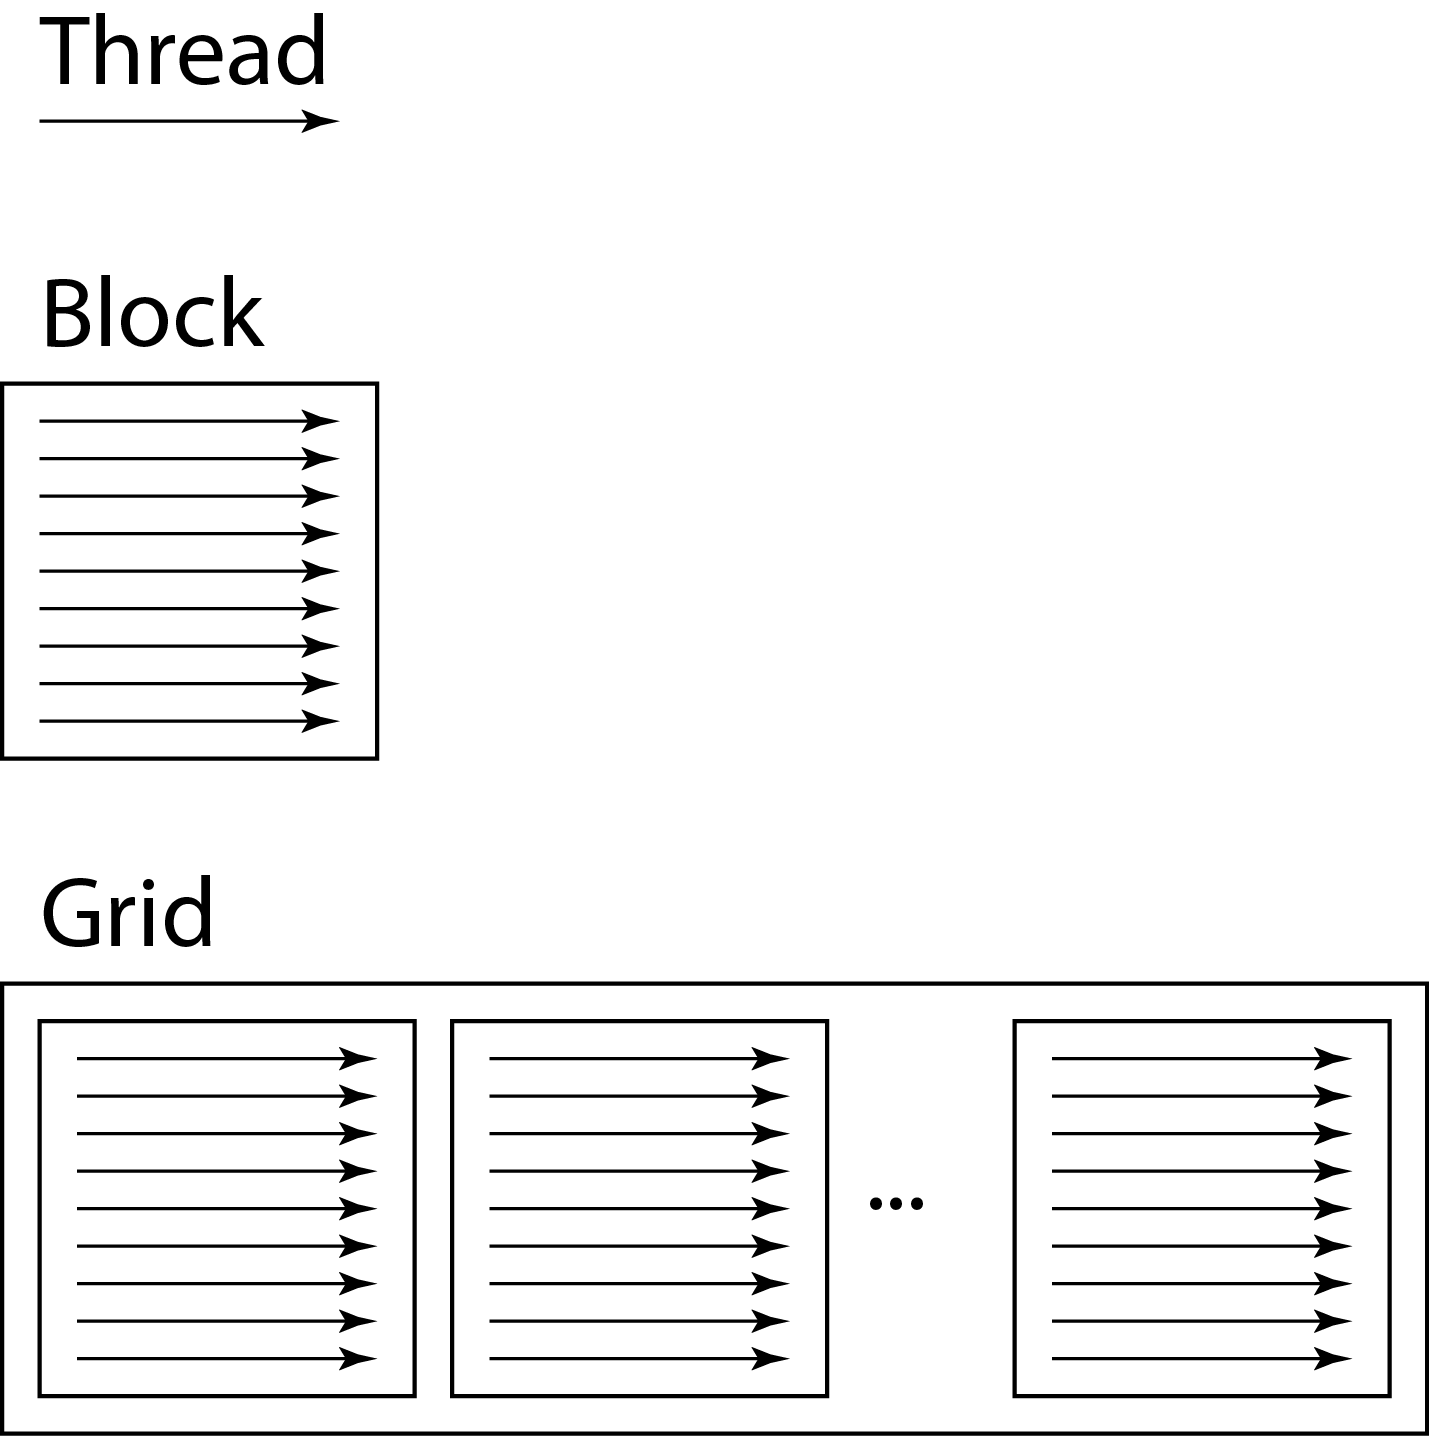
\includegraphics[width=1.0\textwidth,trim=0 0 0 0,clip]{cudastructure.png}}
            \colorbox{white}{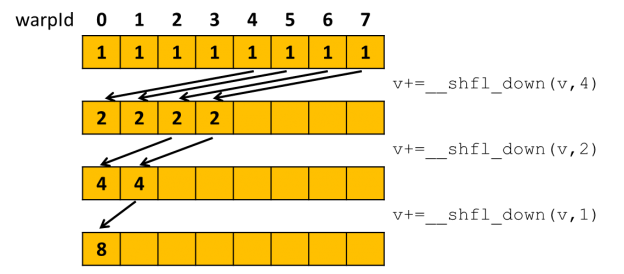
\includegraphics[width=1.2\textwidth,trim=0 0 0 0,clip]{shfl.png}}
            % \caption{}
        \end{figure}
            \end{column}
            \begin{column}{0.7\textwidth}
        \begin{figure}
            \colorbox{white}{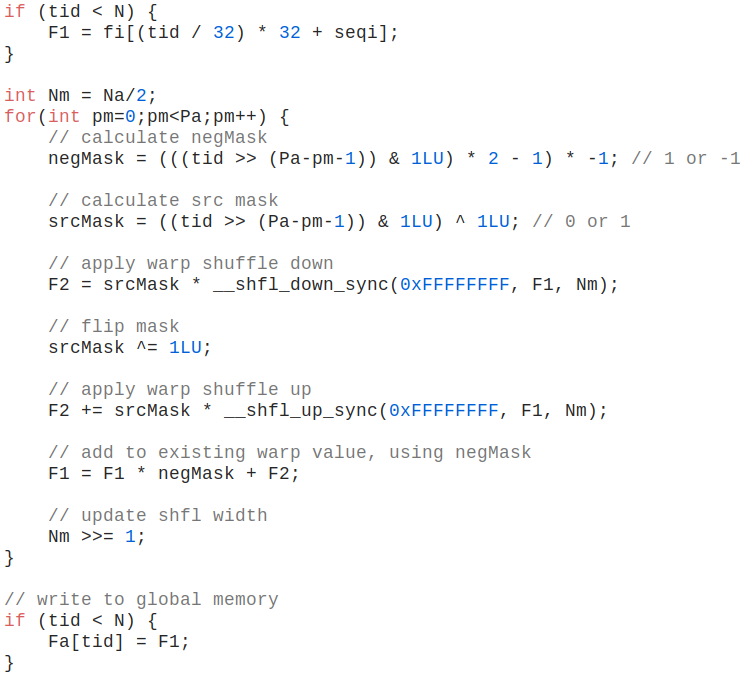
\includegraphics[width=1.0\textwidth,trim=0 0 0 0,clip]{kernel_src.png}}
            % \caption{}
        \end{figure}
            \end{column}
        \end{columns}
    \end{frame}



    \begin{frame}{\mybox{red}{blue}{Results}}
        \vspace{-0.8cm}
        \begin{figure}
            \colorbox{white}{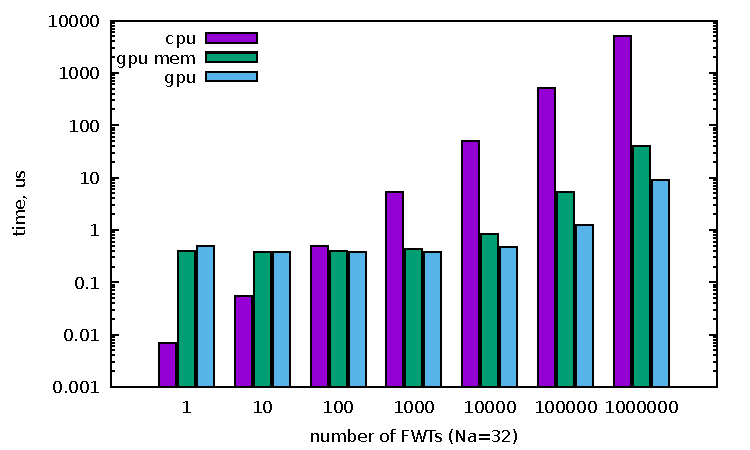
\includegraphics[width=1.0\textwidth,trim=0 0 0 0,clip]{benchmarks.pdf}}
            % \caption{}
        \end{figure}
    \end{frame}

    %%%%%%%%%%%%%%%%%%%%%%%%%%%%%%%%%%%%%%%%%%%%%%%%%%%%%%%%%%%%%%%%%%%%%

    % Bibliography
    %%%%%%%%%%%%%%%%%%%%%%%%%%%%%%%%%%%%%%%%%%%%%%%%%%%%%%%%%%%%%%%%%%%%%
        % \setlength\itemsep{-3pt}
    %%%%%%%%%%%%%%%%%%%%%%%%%%%%%%%%%%%%%%%%%%%%%%%%%%%%%%%%%%%%%%%%%%%%%

  % \end{darkframes}
\end{document}
